\documentclass[titlepage]{article}
\usepackage{babel}
\usepackage{amsmath}
\usepackage{amssymb}
\usepackage{amsthm}
\usepackage{stmaryrd} %ligtning

\usepackage{tabto} %tabulator mit \tab
\usepackage{tikz}
\usetikzlibrary{automata, arrows.meta, positioning, shadows, shapes.geometric} % automaten zeichnen
\usepackage[utf8]{inputenc}
\pagestyle{plain}
\pagenumbering{arabic}
\renewcommand{\arraystretch}{1.3} %vertikaler abstand von tabellen
\usepackage[left=20mm, right=15mm, top=25mm, bottom=7mm, paper=a4paper]{geometry}

\renewcommand{\contentsname}{Inhaltsverzeichnis}
\renewcommand{\]}{\right]}
\renewcommand{\[}{\left[}
\renewcommand{\)}{\right)}
\renewcommand{\(}{\left(}
\renewcommand{\|}{\;|\;}
\newcommand{\n}{\newline}
\renewcommand{\l}{\linebreak}



\begin{document}\begingroup\let\clearpage\relax
	%header
	\begin{center}
	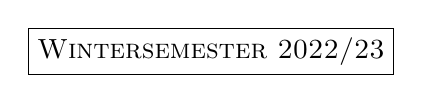
\begin{tikzpicture}
		\draw (0,0) node[draw, rectangle]{\textsc{Wintersemester 2022/23}};
	\end{tikzpicture}
	\hrulefill\\
	\begin{center}
		\LARGE\textsc{Automaten und Berechenbarkeit - Übung 05} \normalsize\\
	\end{center}
	\hrulefill
	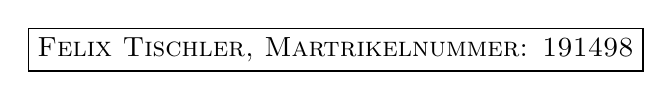
\begin{tikzpicture}
		\draw (0,0) node[draw, rectangle]{\textsc{Felix Tischler, Martrikelnummer: 191498}};
	\end{tikzpicture}
	\date{\today}
\end{center}
	
	%task one
	\section*{Aufgabe 1}
		\include{t1.tex}
		
	\section*{Aufgabe 2}
		\begin{center}
	$M=(\{a,b\},\{A,B,\qedsymbol\},\{Z_0,Z_{ende}\},\delta,Z_0,\{Z_{Ende}\})$\\
\end{center}
Mit:
\begin{center}
	\begin{align*}
		\begin{cases}
			(Z_0,a,\qedsymbol)$&\rightarrow\quad$(Z_0,A\qedsymbol)\\
			(Z_0,a,A)$&\rightarrow\quad$(Z_0,AA)\\
			(Z_0,a,B)$&\rightarrow\quad$(Z_0,\lambda)\\
			(Z_0,\lambda,\qedsymbol)$&\rightarrow\quad$(Z_{ende})\\
			(Z_0,b,\qedsymbol)$&\rightarrow\quad$(Z_0,B\qedsymbol)\\
			(Z_0,b,A)$&\rightarrow\quad$(Z_0,\lambda)\\
			(Z_0,b,B)$&\rightarrow\quad$(Z_0,BB)
		\end{cases}
	\end{align*}
\end{center}
	
\endgroup\end{document}